% COMP3314 Group Project report, Group 35
% Paper: van der Maaten & Hinton (2008), Visualizing Data using t-SNE, JMLR 9.
% Limits: max 4 pages main text (references and appendix excluded). Due 29 Nov 2026, 23:59, as PDF named Group_35.
%
% Suggested page budget (4.0 pages in total; change it together, not alone):
%   Abstract 0.1 | 1 Introduction 0.5 | 2 Method 1.0 | 3 Experiments in the paper 0.5
%   4 Critical analysis 0.9 | 5 Reproduction 0.8 | 6 Conclusion 0.2
%
% Rule from the brief: label every figure and number as the paper's or ours.

\documentclass{article}

% Course template: NeurIPS 2026 style (official neurips_2026.sty, kept in extra/), preprint option.
% Build: tectonic -X compile -Z search-path=extra report.tex (VS Code does this on save).
\PassOptionsToPackage{numbers, compress}{natbib}
\usepackage[preprint]{neurips_2026}

\usepackage[utf8]{inputenc}
\usepackage[T1]{fontenc}
\usepackage{hyperref}
\usepackage{url}
\usepackage{booktabs}
\usepackage{array}       % appendix table (B4)
\usepackage{amsmath,amssymb,amsfonts}
\usepackage{graphicx}
\usepackage{xcolor}

% Read figures straight from where they are generated (do not copy or edit them there).
%   resources/figures/            E1-E7, small digits set
%   submission/outputs/compare3/  the 12 maps on MNIST, Olivetti, COIL-20
%   submission/outputs/figures/   E8, MNIST-6000
%   report/figures/               B4 critical analysis (method map; sizes and gaps), drawn in TikZ, sources in figures/source/
\graphicspath{{../../resources/figures/}{../outputs/compare3/}{../outputs/figures/}{figures/}}

\title{Visualizing Data using t-SNE: Study, Critical Analysis and Partial Reproduction}

% TODO (each member): check the spelling of your name; add an email line if we want one.
\author{%
  Jelisaveta Vasiljevic \\
  The University of Hong Kong
  \And
  Alexandre Bommensath \\
  The University of Hong Kong
  \And
  Anna Claire Breuss-Burgess \\
  The University of Hong Kong
  \And
  Adel Kussainova \\
  The University of Hong Kong
}

\begin{document}

\maketitle

\begin{abstract}
  % TODO (joint, write last, about 5 sentences):
  % the paper and its problem; the key idea (heavy-tailed Student-t map kernel);
  % our verdict on the evidence; what we reproduced and the headline number.
\end{abstract}

\section{Introduction}
% Owner: B1. Target: 0.5 page.
% Problem formulation, motivation, main contributions of the paper.

\section{Method}
\label{sec:method}
% Owner: B2, Anna Claire. Target: 1.0 page.
% SNE, symmetric SNE, the crowding problem, Student-t kernel, gradient, optimisation tricks.
% Connections to course topics.

\section{Experiments in the paper}
\label{sec:evidence}
% Owner: B3, Alex. Target: 0.5 page.
% Setup (MNIST, Olivetti, COIL-20), baselines, what the evidence supports.

\section{Critical analysis}
\label{sec:critical}
% Owner: B4, Jelisaveta. Figures 1-2 and the claims table are in Appendices A-B.
% Conventions: \S = a section of the paper; "our Section" = this report; "step" = Figure 1.


We judge the paper in its own order: the argument, the method, the experiments and claims, and what came after. From the method on, we name its strengths (S), the assumptions it never checks (A) and its limitations (L), each backed by the paper, our own experiments or later work. These labels, and the steps of the method we refer to (``step~1'' to ``step~4''), come from Figure~\ref{fig:map} in Appendix~\ref{app:map}, which places each S, A and L under the step that causes it; we recommend reading this section alongside it. References with \S\ are to sections of the paper; ``our Section'' and ``Appendix'' refer to this report, and numbers marked ``ours'' come from our own experiments.

\paragraph{1. The argument: is it sound?}
The main problem is crowding, as SNE and Sammon mapping squeeze points at moderate distance into the middle of the map. The authors show its cause, too little room in a 2-D map (\S3.2), and fix that cause with a heavy-tailed curve on the map (\S3.3), whereas the earlier fix they discuss, UNI-SNE, only eased the symptom. Our own test supports the fix: with a Gaussian curve instead, the 1-NN error on digits rises from 1.9\% to 8.2\% (our Section~\ref{sec:repro}). Each link follows from the last and the fix targets the cause, not its effect, so the argument is sound.

\paragraph{2. The method: does it work?}
\textbf{The central trade-off.} t-SNE is built to keep neighbours, not distances, through two design choices (our Section~\ref{sec:method}): step~1 gives every point about the same number of neighbours, set by one fixed perplexity, and the cost in step~3 punishes a lost neighbour heavily but barely weighs far-apart pairs. Because far pairs barely count, the heavy-tailed curve of step~2 can push moderately distant points apart without penalty, so t-SNE fixes crowding at its cause (S1). Because a lost neighbour costs the most, t-SNE keeps true neighbours best (S2): its map classifies about as well as the raw images (1-NN error 5.13\% against 5.75\% in \S5; ours 5.92\% against 6.03\%) and far better than its rivals (our Section~\ref{sec:repro}). The same two choices cause the main limitation: group sizes and gaps are distorted (L1). With equal neighbour counts, a wide group and a tight group look alike in $P$, so sizes are lost; with far pairs barely counting, the map may place distant groups almost anywhere, so gaps are lost. On synthetic clusters, one 5.1 times as wide as another is drawn the same size, while PCA keeps the ratio (Figure~\ref{fig:sizes}, Appendix~\ref{app:claims}). The authors present this design only as an advantage (\S2); we see L1 as the price of S1 and S2.

\textbf{Assumptions.} The map is built from the neighbours chosen in step~1, so if they are wrong, the map is wrong too. Step~1 rests on three choices the paper never tests. Cutting the data to 30 dimensions with PCA (Lecture~3) assumes this loses nothing important (A3, \S4.2), yet PCA is linear and can blur curved structure that separates neighbours. Choosing neighbours by straight-line distance assumes that close means similar (A1), yet two face photos of different people in similar light can be closer in pixels than two of the same person; the authors themselves doubt this for faces (\S6.2). Using one perplexity for every point assumes that one neighbour count fits all groups (A2), yet a small group may need fewer neighbours than a large one. Each could fail on real data, so each should be tested (Extension~2).

\textbf{Other strengths and limitations.} t-SNE is also easier to run than SNE (S3), with a simpler gradient and no simulated annealing (\S3.1, \S3.3). Its remaining limitations are practical, and the authors admit them. Because each run starts at random and depends on settings such as the perplexity, the layout changes between runs (L2): across our seeds and perplexities the quality stayed the same (1-NN error 1.9--2.3\%), but the groups moved and changed shape. Using every pair at every step makes it slow on big data (L3, $O(n^2)$); learning no mapping, it cannot add new points (L4); and with the tail's weight set by hand, it is only shown for 2-D and 3-D maps (L5, \S6.2). Overall, the method is strong, with one built-in trade-off: keeping neighbours gives S1 and S2 and causes L1, the maps are only as good as A1--A3 allow, and the other limits concern running it, not what its maps mean; since most were fixed later (part~4), they weigh little against the method.

\paragraph{3. The experiments and claims: do they hold?}
\textbf{The experiments.} The experiments are wide and honest (S4): seven rival methods on five data sets, with the weaknesses stated (\S6.2). But they are judged by eye, with no score (L6), one setting per rival. Only \S5 uses a score, the 1-NN error; in our reproduction it is 3.6--6.3\% for t-SNE and 18.8--64.3\% for the three rivals we reran on the three main data sets (our Section~\ref{sec:repro}). The pictures were right, but the paper never measured it.

\textbf{The claims.} Our Section~\ref{sec:evidence} rates the paper's own evidence; adding our own tests, of the paper's seven claims (Appendix~\ref{app:claims}), two hold: true neighbours are kept (measured, as long as A1 holds), and crowding is reduced, shown by eye and backed by our Gaussian test. Three rest only on pictures, with no score: structure at many scales (the paper's Figure~7), very large data sets (one map of 6{,}000 digits) and beating every rival (the side-by-side maps of \S4). Two are never measured by the paper: easier optimisation, argued from the gradient without runs against SNE, and stability between runs, stated (\S6.2) without repeated runs; our runs show stable quality but a moving layout. Our score has a limit too: it measures only whether neighbours are kept, exactly what t-SNE is built for, so it cannot show that t-SNE is better overall. Overall, the core holds, but the broad claims overreach.

\paragraph{4. After the paper: what was fixed?}
The practical limits were largely fixed, and t-SNE became a standard tool~\cite{sklearn}. Two are solved by default today: Barnes--Hut, which treats far-away groups of points as one, fixes L3~\cite{vdm14}, and starting the map from a PCA layout instead of at random fixes L2~\cite{kl21}. Three more have fixes that are not standard: parametric t-SNE, a neural network that places new points and learns the tail's weight for more dimensions (L4, L5~\cite{vdm09}), and density-preserving t-SNE, which adds a cost term that keeps group sizes (L1~\cite{nbc21}). One assumption can be avoided: combining several neighbourhood sizes removes the need for one perplexity (A2~\cite{lee15}). Still open are judging maps by eye rather than by a score (L6), the untested A1 and A3, and the lack of a theory of when t-SNE works (L7), since proofs cover only well-separated clusters~\cite{ahk18,ls19}. Overall, t-SNE is partly fixed, and widely used: what limits running it is solved, but what limits reading its maps is not.

\paragraph{5. Verdict.}
The argument is sound and the method strong: keeping neighbours rather than distances fixes crowding and keeps true neighbours together. That same choice brings the one caution, that the maps cannot show how large groups are or how far apart they lie. The core claims hold, but the broader ones rest only on pictures, and the practical limits have since been largely fixed. Therefore, taking the four parts together, this is a good, lasting paper, with one caution: a t-SNE map should be read for which groups exist, not for their sizes or the distances between them~\cite{wat16}.

\paragraph{6. Extensions.}
Each extension addresses a gap that is still open. \textbf{(1) Score the comparison (L6).} The paper judges its rivals by eye, so we would tune every rival, repeat over seeds, and score how well each map keeps both neighbours and group sizes; this would test ``better than every rival'', which we expect t-SNE to win on neighbours only. \textbf{(2) Test the assumptions (A1--A3).} On Olivetti our map makes more errors than the raw images (25 against 20 in 400), perhaps because an assumption fails. We would rerun it three times, changing one thing each time: no PCA step (A3), neural-network features instead of raw pixels (A1, as \S6.2 suggests), and a different perplexity per group (A2~\cite{lee15}); the change that closes the gap shows which assumption failed, if any. \textbf{(3) Show the sizes the map drops (L1).} In step~1, t-SNE computes a width $\sigma_i$ for every point, larger where its group is more spread out, and then discards it, yet on our clusters these widths keep most of the true size ratio (4.1 and 5.0 against 5.1; Figure~\ref{fig:sizes}). Colouring each point by its $\sigma_i$ would let a reader judge which groups are truly spread out or tight, even where the map draws them the same size, helping to correct the main misreading of t-SNE maps without changing the method.

\section{Reproduction}
\label{sec:repro}
% Owner: B3, Alex. Target: 0.8 page.
% Scope, implementation, comparison with the paper, discrepancies and challenges.
% Code (the link must appear in the text): \url{https://github.com/LizaaV/tsne-from-scratch}
% Label our results clearly as ours, and figures taken from the paper as the paper's.
% Our numbers: submission/outputs/compare3/REPORT.md.

\section{Conclusion}
% Joint. Target: 0.2 page. Verdict on the paper, and what we learned.

% TODO: add the other sources we cite (SNE, Sammon, Isomap, LLE, and the later t-SNE work).
\begin{thebibliography}{9}
\bibitem{vandermaaten2008}
L.~van der Maaten and G.~Hinton.
\newblock Visualizing data using t-{SNE}.
\newblock \emph{Journal of Machine Learning Research}, 9(86):2579--2605, 2008.

% Later work cited in Section 4 (B4).
\bibitem{vdm14} L.~van der Maaten. Accelerating t-SNE using tree-based algorithms. \emph{JMLR}, 15(93):3221--3245, 2014.
\bibitem{vdm09} L.~van der Maaten. Learning a parametric embedding by preserving local structure. In \emph{AISTATS}, PMLR 5:384--391, 2009.
\bibitem{wat16} M.~Wattenberg, F.~Vi\'egas, and I.~Johnson. How to use t-SNE effectively. \emph{Distill}, 2016. doi:10.23915/distill.00002.
\bibitem{kl21} D.~Kobak and G.~C. Linderman. Initialization is critical for preserving global data structure in both t-SNE and UMAP. \emph{Nature Biotechnology}, 39:156--157, 2021.
\bibitem{ahk18} S.~Arora, W.~Hu, and P.~K. Kothari. An analysis of the t-SNE algorithm for data visualization. In \emph{COLT}, PMLR 75:1455--1462, 2018.
\bibitem{ls19} G.~C. Linderman and S.~Steinerberger. Clustering with t-SNE, provably. \emph{SIAM J. Math. Data Sci.}, 1(2):313--332, 2019.
\bibitem{lee15} J.~A. Lee, D.~H. Peluffo-Ord\'o\~nez, and M.~Verleysen. Multi-scale similarities in stochastic neighbour embedding: reducing dimensionality while preserving both local and global structure. \emph{Neurocomputing}, 169:246--261, 2015.
\bibitem{nbc21} A.~Narayan, B.~Berger, and H.~Cho. Assessing single-cell transcriptomic variability through density-preserving data visualization. \emph{Nature Biotechnology}, 39:765--774, 2021.
\bibitem{sklearn} F.~Pedregosa et al. Scikit-learn: machine learning in Python. \emph{JMLR}, 12(85):2825--2830, 2011.
\end{thebibliography}

% Appendices (excluded from the 4-page limit). A and B belong to Section 4.
\appendix

\section{Method map of our critical analysis}
\label{app:map}

Figure~\ref{fig:map} is the map for Section~\ref{sec:critical}. The boxes are the steps of t-SNE (our Section~\ref{sec:method}); each label below a box is a strength, assumption or limitation that comes from that step, and the dashed strip holds those about the paper as a whole.

\begin{figure}[!h]
  \centering
  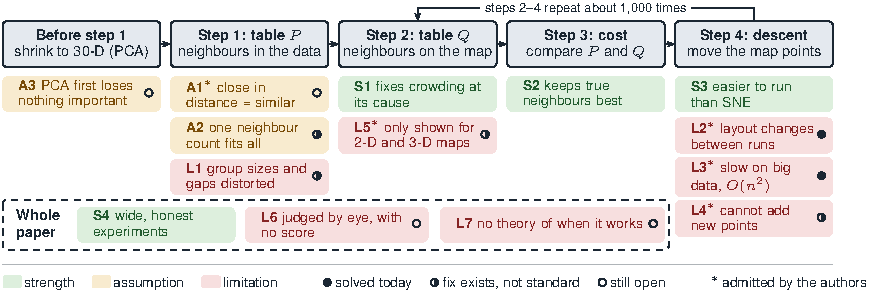
\includegraphics[width=\linewidth]{B4_method_map.pdf}
  \caption{Our critical analysis at a glance (our figure): the steps of t-SNE, and each strength (S), assumption (A) and limitation (L) under the step that causes it. The dot shows its state today, and $^*$ marks those the authors admit themselves.}
  \label{fig:map}
\end{figure}

\section{The paper's claims, and the synthetic-cluster test}
\label{app:claims}

\subsection{The seven claims}
\label{app:claims-table}

Table~\ref{tab:claims} supports the count in Section~\ref{sec:critical}. Verdicts use the paper, our experiments (Sections~\ref{sec:critical} and~\ref{sec:repro}) and later work.

\begin{table}[!h]
\centering\footnotesize
\caption{Seven claims, how the paper supports them, and our verdict.}
\label{tab:claims}
\begin{tabular}{@{}>{\raggedright}p{0.25\linewidth}>{\raggedright}p{0.25\linewidth}>{\raggedright}p{0.27\linewidth}>{\raggedright\arraybackslash}p{0.125\linewidth}@{}}
\toprule
Claim (where) & Paper's evidence & What we add & Verdict \\
\midrule
Less crowding (abstract, \S3) & cause explained; maps judged by eye & Gaussian map kernel: 1-NN error 1.9\% $\to$ 8.2\% & holds \\
Captures local structure (\S1) & 1-NN error 5.13\% on the map, 5.75\% on pixels (\S5) & 5.9\% against 6.0\% on MNIST; Olivetti slightly worse than raw & holds, if A1 holds \\
Many scales in one map (abstract) & pictures (Fig.~7) & sizes and gaps distorted (Figure~\ref{fig:sizes}) & by eye \\
Very large data sets (abstract, \S5) & 6{,}000 of 60{,}000 digits drawn (Fig.~7) & not reproduced & by eye \\
Better than other techniques (abstract, \S7) & 40 maps, one setting per rival (Table~1 of the paper) & better at neighbours than three rivals; PCA better at sizes & by eye \\
Easier to optimise than SNE (abstract, \S3.3) & argued from the gradient & not tested: we did not run SNE & not tested \\
Quality stable between runs (\S6.2) & stated, no runs shown & five seeds on digits: $2.1\pm0.1\%$, layout moves & not tested by the paper \\
\bottomrule
\end{tabular}
\end{table}

\subsection{The synthetic-cluster test}
\label{app:sizes}

Figure~\ref{fig:sizes} backs limitation L1 and Extension~(3) in Section~\ref{sec:critical}: on clusters whose sizes and gaps are known, it compares what PCA and t-SNE draw.

\begin{figure}[!h]
  \begin{minipage}[c]{0.52\linewidth}
    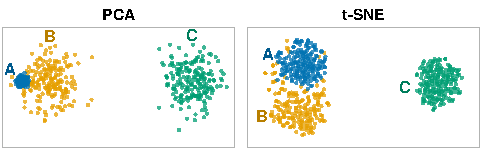
\includegraphics[width=\linewidth]{B4_sizes_gaps.pdf}
  \end{minipage}\hfill
  \begin{minipage}[c]{0.46\linewidth}
    \footnotesize\setlength{\tabcolsep}{3pt}\centering
    \begin{tabular}{@{}lcccc@{}}
      \toprule
      & true & PCA & t-SNE & $\sigma_i$ \\
      \midrule
      width B/A & 5.1 & 5.4 & \textbf{1.4} & 4.1 \\
      width C/A & 5.1 & 5.5 & \textbf{1.0} & 5.0 \\
      gap BC/AB & 5.2 & 5.2 & \textbf{3.4} & -- \\
      \midrule
      1-NN error (digits) & 2.5\% & 42.5\% & \textbf{1.9\%} & -- \\
      \bottomrule
    \end{tabular}
  \end{minipage}
  \caption{Our results: three synthetic 10-D clusters A, B, C with known sizes (one run). Widths and gaps are ratios between clusters; the $\sigma_i$ column is the ratio of the clusters' median bell widths from step~1. Last row: 1-NN error on the small digits set (1{,}797 images; true = raw pixels). PCA keeps sizes and gaps, t-SNE keeps neighbours.}
  \label{fig:sizes}
\end{figure}

\paragraph{How it was made.} Three Gaussian clusters of 200 points in 10-D: A has standard deviation 1, B and C have 5, and the centres lie at distances 10 (A to B) and 50 (B to C). t-SNE uses our implementation, perplexity 30, no PCA, seed 0. Width is the mean distance of a cluster's points to their centre; gap is the distance between centres; the $\sigma_i$ column is the ratio of the clusters' median $\sigma_i$. Pairs that join B and C hold less than $10^{-6}$ of the total mass of $P$. The $\sigma_i$ ratio for B/A (4.1) is below the true 5.1 because B overlaps A, so some neighbours of B's points lie in the tight cluster.

\end{document}
